\subsection*{ГЛ11 6}
Отметим точку $S \notin a,b$. Затем проведем $SA,\ SA \cap a = K,\ SA \cap b = K'$. Произвольно проведем $SL, SN$, где $SL \cap a = L,\ SL \cap b = L'$. Теперь проведем $AL,AL'$ и $SN \cap AL = N,\ SN \cap AL' = N'$. Пусть $KN \cap K'N' = C$, тогда $AC$ -- искомая прямая, так как $A,B,C$ на одной прямой.\\
\begin{figure}[h]
	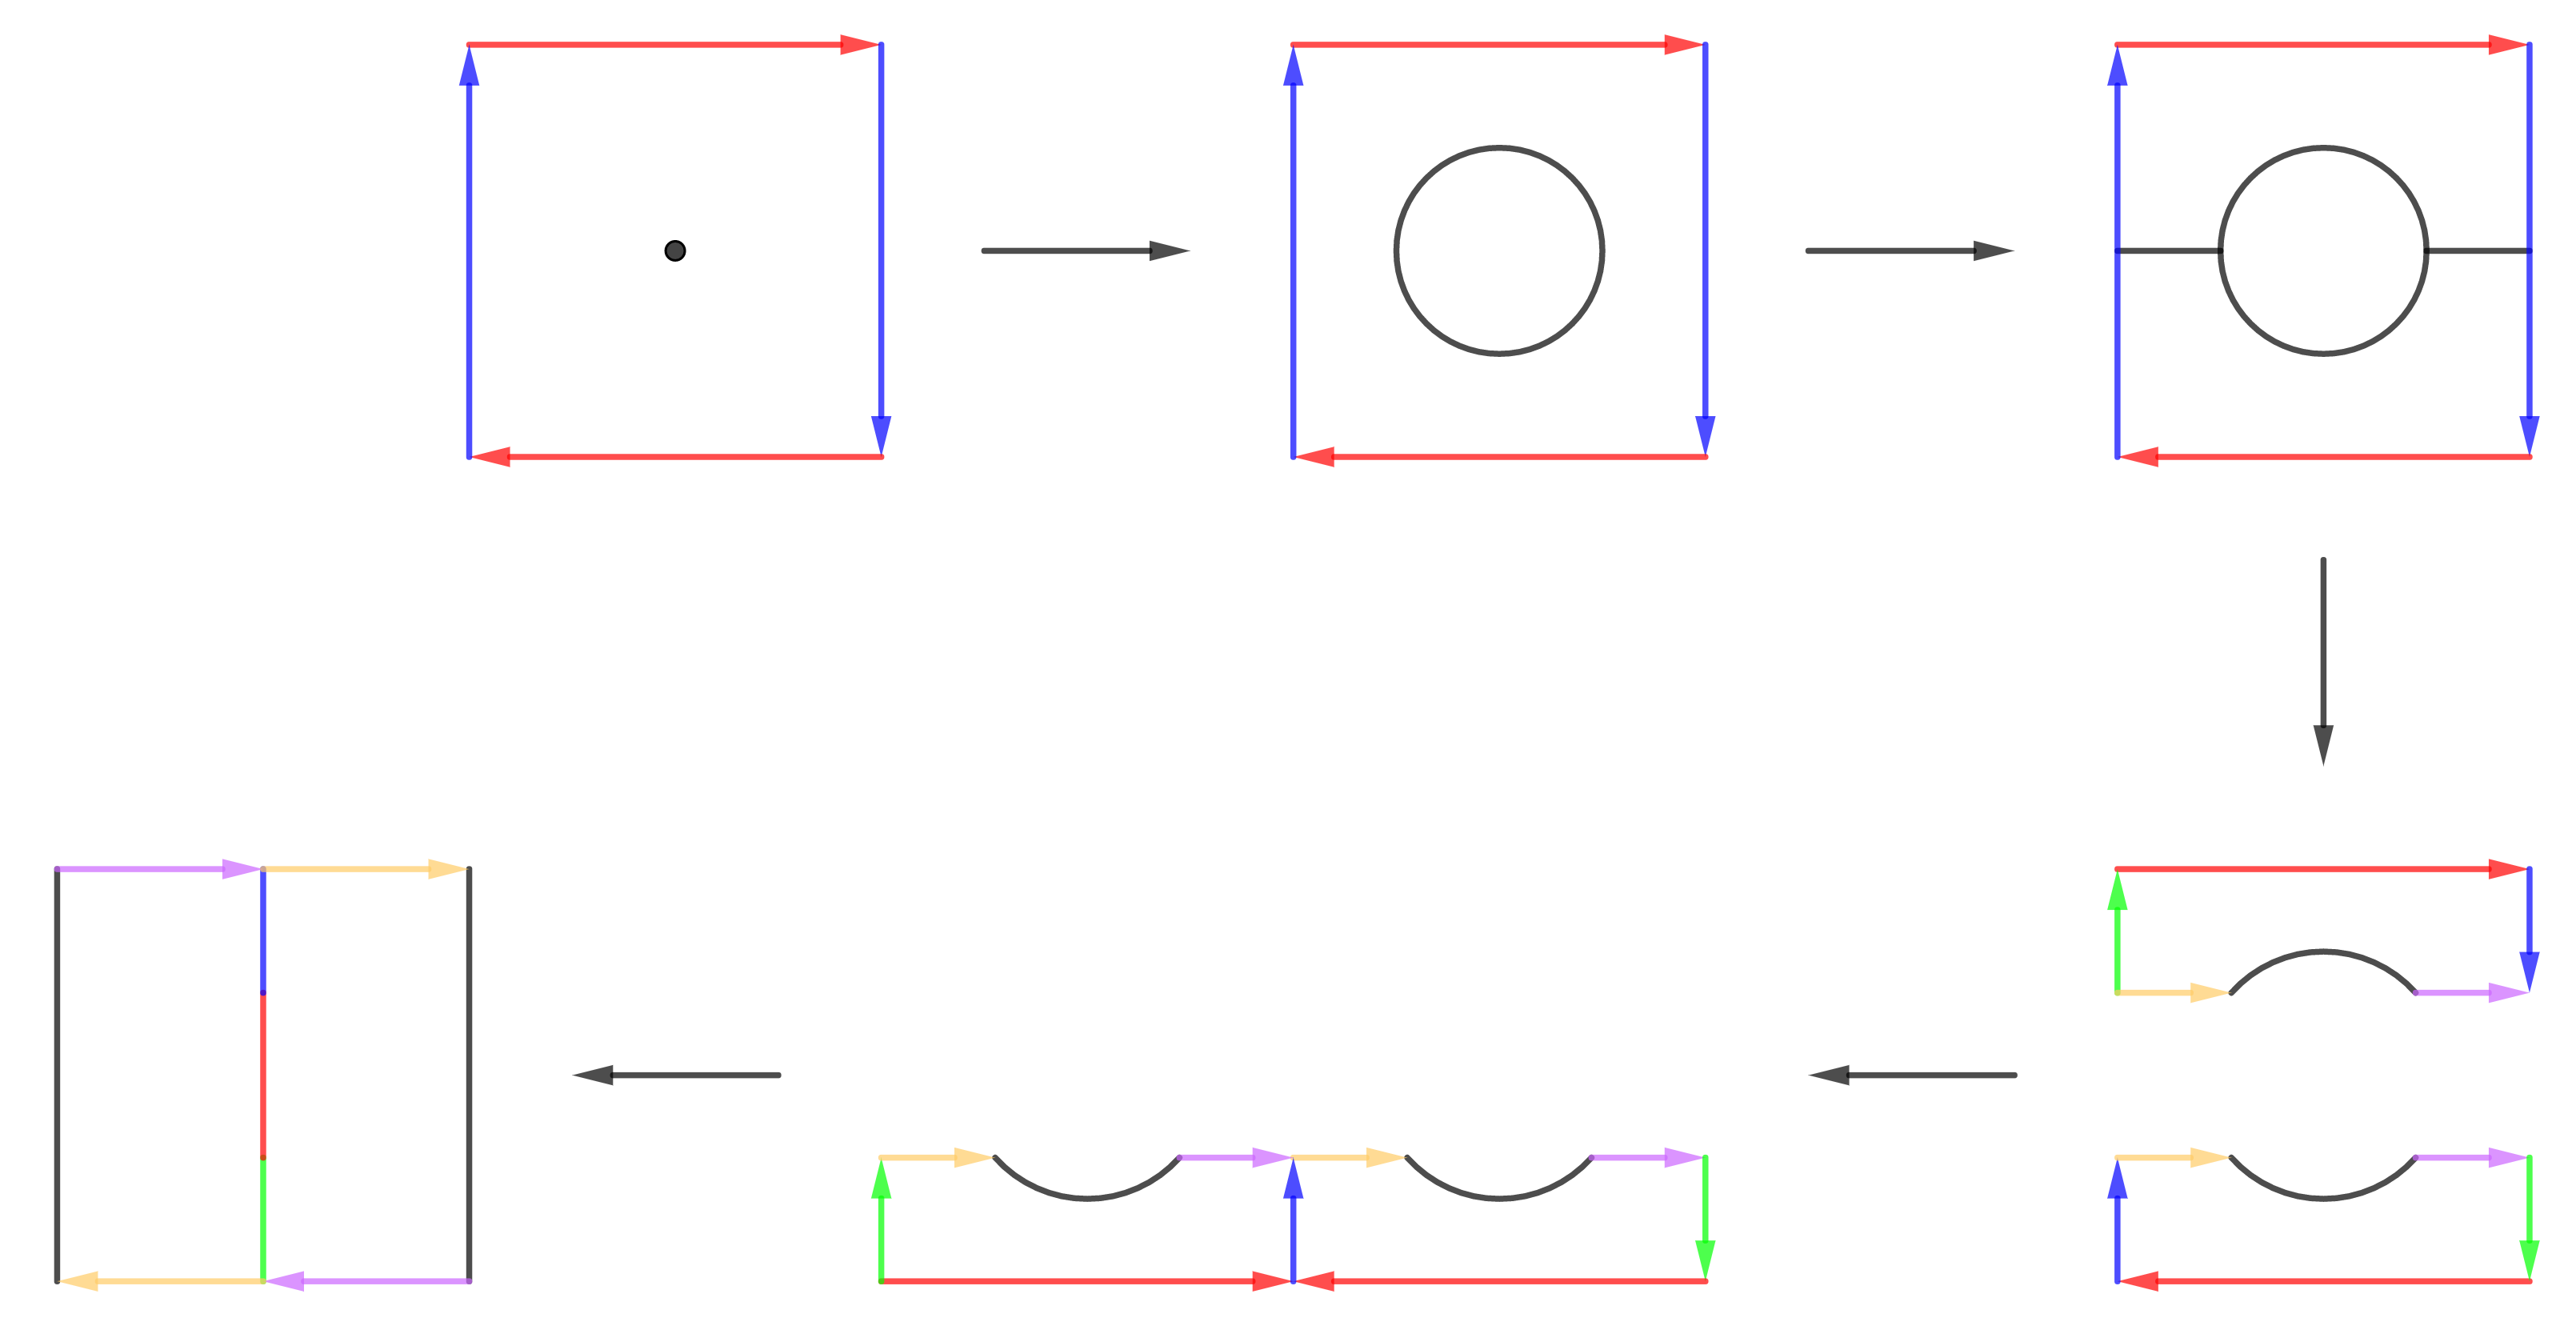
\includegraphics[width=0.4\linewidth]{pic4}
\end{figure}
Докажем корректность построения. $\triangle NCN'$ и $\triangle L'LB$ перспективные. Тогда так как $NN' \cap LL'= S,\ NC \cap BL = K,\ NÇ \cap BL'= K'$ и $S,K,K'$ на одной прямой по построению, то $NL, BC, N'L'$ пересекаются в одной точке $NL \cap N'L' = A$ по построению, то $A,B,C$ лежат на одной прямой
		
		